\chapter{Radioactivity}

\section{Units}

Before we begin, a quick note on units: 

\begin{enumerate}
\item Nuclear sizes are typically of order $10^{-15} \, {\rm m}$ (1 fm).
\item Nuclear time scales have a vast range, e.g. half-life can range from $10^{-20} \, {\rm s}$ to greater than the age of the Universe!
\item Nuclear energies are typically measured in MeV, where $1 \, {\rm eV} = 1.602 \times 10^{-19} \, {\rm J}$.
\item Nuclear masses are typically measured in the unified atomic mass unit (u), defined such that the mass of a Carbon-12 atom = 12 u. In terms of SI units, $1\,{\rm u} = 1.66054 \times 10^{-27}\,{\rm kg}$.

A Carbon-12 nucleus has 6 protons and 6 neutrons. Nucleons therefore have a mass of around 1 u (since the mass of the electron is much smaller than the mass of the proton and neutron, and the mass of protons/neutrons are approximately the same), where $1 \, {\rm u} = 931.5 \, {\rm MeV}/{\rm c}^2$. Note I have now defined the mass in terms of energy divided by $c^2$, using the fact that $E=mc^2$. This is useful as we will commonly multiply masses by $c^2$ to obtain the energy, and the factors of $c$ will therefore cancel.

As an example, the proton has a mass of $m_p = 1.673 \times 10^{-27}\,{\rm kg}$ in SI units. This is equal to $m_p = 938.3\,{\rm MeV/c^2}$. The neutron has a mass of $m_n = 1.675 \times 10^{-27}\,{\rm kg}$ in SI units. This is equal to $m_n = 940.6\,{\rm MeV/c^2}$.

\end{enumerate}

{\em Working in these units will make calculations easier and will be less likely to lead to mistakes.} %It also allows us to quickly determine if the energy is greater than the (rest) mass of a particle, in which case we need to include relativistic effects.  

\section{Radioactive decay}

The nucleus consists of protons (positively charged) and neutrons (neutral), which have approximately the same mass (the mass difference is important however in calculations!). Isotopes are defined as having different numbers of neutrons. Deuterium, for example (those nucleus consists of 1 proton and 1 neutron), is an isotope of hydrogen. 

\begin{definition}{Radioactive Decay}
The spontaneous emission of radiation(s) that changes the state of the nucleus.
\end{definition}

\begin{definition}{Nuclear notation}
We will define a nucleus by
\beq
^A_Z {\rm X}\,,
\eeq
where $Z$ is the proton number (also called the atomic number) and $A=Z+N$ is the mass number, where $N$ is the number of neutrons. $X$ is the name of the nucleus, and is unique for a given $Z$. The $Z$ number is therefore sometimes omitted for common nuclei. 
\end{definition}

Radioactivity was discovered in 1896 by Henri Becquerel when he realised that Uranium was darkening a photographic plate in a cupboard.  The Curies discovered more radioactive materials and realised there were three types of decay:

\begin{description}
\item[Alpha decay ($\alpha$) ] A helium nucleus (2 protons and 2 neutrons) is emitted from a parent nucleus. It is strongly ionising, heavy (compared to the other types of radioactive decay), and has a charge of $+2e$. It is very damaging if inside the body.
\item[Beta decay ($\beta$)] A high energy electron or positron (the anti-particle of an electron) is emitted from the nucleus. In the case of an electron being emitted (sometimes called $\beta^-$ decay), a neutron in the parent nucleus decays into a proton and an electron (plus an electron anti-neutrino). It is less ionising than $\alpha$ decay, but has a much faster speed, with lower charge ($-e$ or an electron or $+e$ for a positron). In the case of a positron being emitted (sometimes called $\beta^+$ decay), a proton in the parent nucleus decays into a neutron and a positron (plus an electron neutrino).
\item[Gamma decay ($\gamma$)] The nucleus de-excites and emits a gamma ray photon (like electron transitions leading to photons in atoms). It is very energetic, interacts weakly with matter, and is uncharged.
\end{description}

\begin{figure}[h!]
\centering
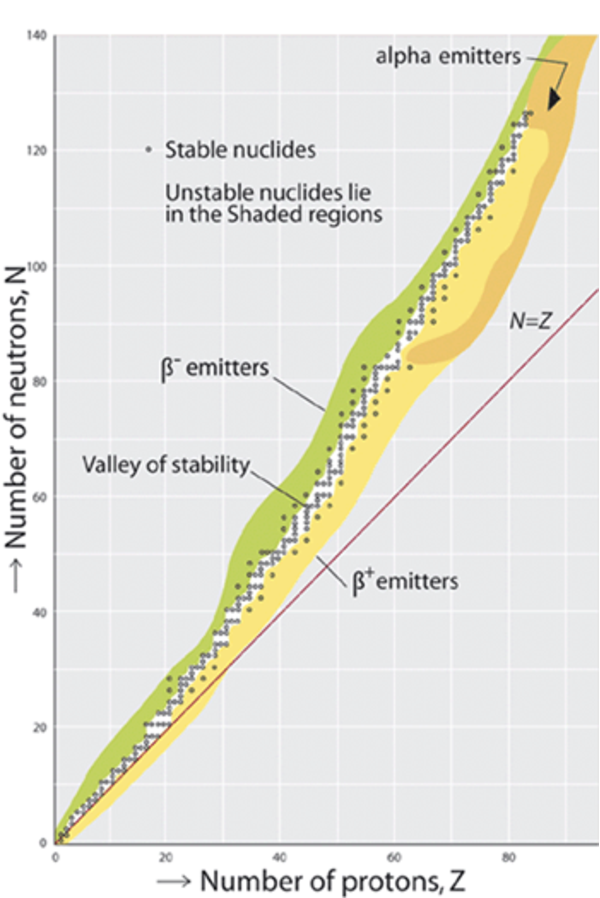
\includegraphics[width=0.6\columnwidth]{plots/stability.pdf}
\caption{\label{fig:stability} Segre chart.}  
\end{figure}

We will discuss each of these in more detail shortly. Of about 2500 known nuclides, only about 300 are stable.  The stable nuclei form a narrow distribution on a plot of $N$ versus $Z$, as shown in Fig.~\ref{fig:stability}.  This plot is known as a Segre chart. The stability valley moves away from the $N=Z$ line for large $Z$. Larger nuclei need more neutrons relative to protons to remain stable, since neutrons are uncharged and have no repulsive Coulomb forces.  

 Nuclei can decay by either alpha or beta emission to move from the unstable regions towards the stable valley. To move on this diagram they must change $N$ or $Z$ or both.  Heavier nuclei tend to decay by $\alpha$ decay, and lighter nuclei tend to decay by beta emission (those with a neutron excess decay by $\beta^{-}$ emission and those with a proton excess by $\beta^{+}$ emission). No nuclide with $A>209$ or $Z>83$ (Bismuth, Bi) is stable.
